\documentclass{article}
\usepackage[utf8]{inputenc}
\usepackage{natbib}
\usepackage[T1]{fontenc}
\usepackage[francais]{babel}
\usepackage{chemist}
\usepackage{array}
\usepackage[version=3]{mhchem}
\usepackage{amsmath}
\usepackage[squaren,Gray]{SIunits}
\usepackage{numprint}
\usepackage{amsfonts}
\usepackage{amssymb}
\usepackage{graphicx}
\usepackage{mathtools}
\usepackage{fullpage}
\usepackage{mhchem}
\usepackage{listings}
\usepackage{hyperref}
\usepackage{mathenv} %%%%%%%%%%% do not forget to add to head.tex
\usepackage{empheq} %%%%%%%%%%%% same
\author{Groupe 1246 }


\begin{document}
\section*{Comparaison entre le modèle de notre outil de gestion et celui de Aspen+}
Il nous a été demandé dans le cadre de la seconde tâche d'analyser plus précisément la dernière étape du procédé, le réacteur de production d'ammoniac, considéré comme une "une boite noire" depuis le début du projet. Une analyse paramétrique a été réalisée avec notre outil de gestion ainsi qu'avec le logiciel Aspen+. Ce document présente les résultats et conclusions de cette dernière ainsi que la comparaison des modèles obtenus à l'aide des deux procédés.

\subsection{Adaptation de la réaction: état d'équilibre}
La réaction est la suivante:

$$N_{2(g)} + 3H_{2(g)} \Leftrightarrow NH_{3(g)}$$

Nous avons durant la première tâche faussement considéré que cette réaction était complète. Nous avons donc dans un premier temps calculé un degré d'avancement afin de savoir précisement combien de moles de $NH_3$ était réellement produite. 

tab + calcule.
\subsection*{analyse paramétrique: outil de gestion.}
Suite à cela, nous avons codé une fonction "synthese(N,H,A,T,p)" calculant le nombre de tonne de NH3 produite en fonction des quantité de réactif, de la témpérature et de la pression. Une première étude paramétrique a été réalisée pour une production théorique de \unit{1500}{\tonne}, pour des températures allant de \unit{0}{\celsius} à \unit{1500}{\celsius}, et pour des pressions allant de \unit{0}{bars} à \unit{250}{bars}. Les graphiques obtenus sont les suivants:

\begin{figure}[ht!]
 \centering
 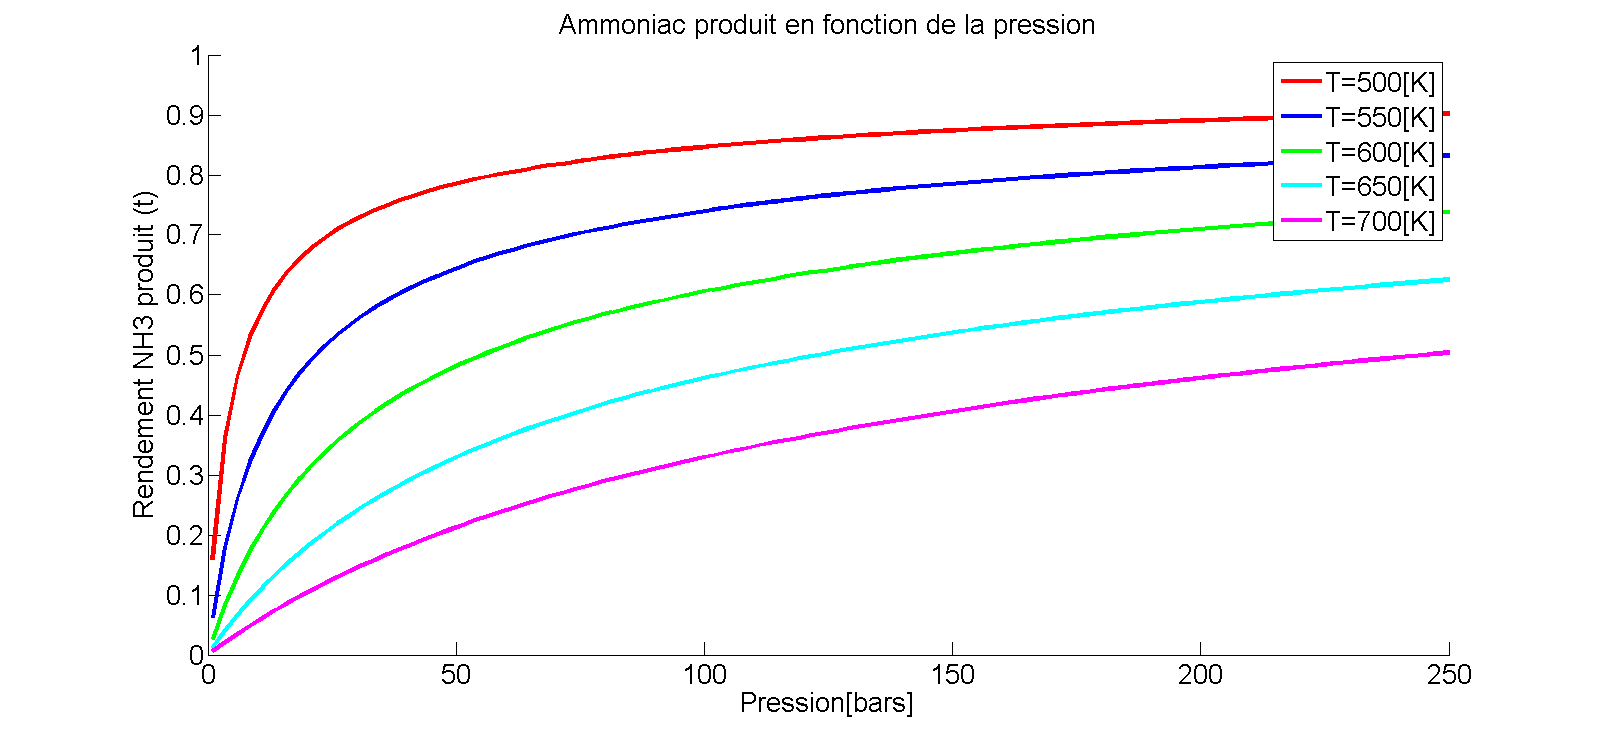
\includegraphics[scale=0.2]{GrapheNH3P.png}
 \caption{Evolution du rendement en fonction de la pression}
 \label{scheme1}
\end{figure}

\begin{figure}[ht!]
 \centering
 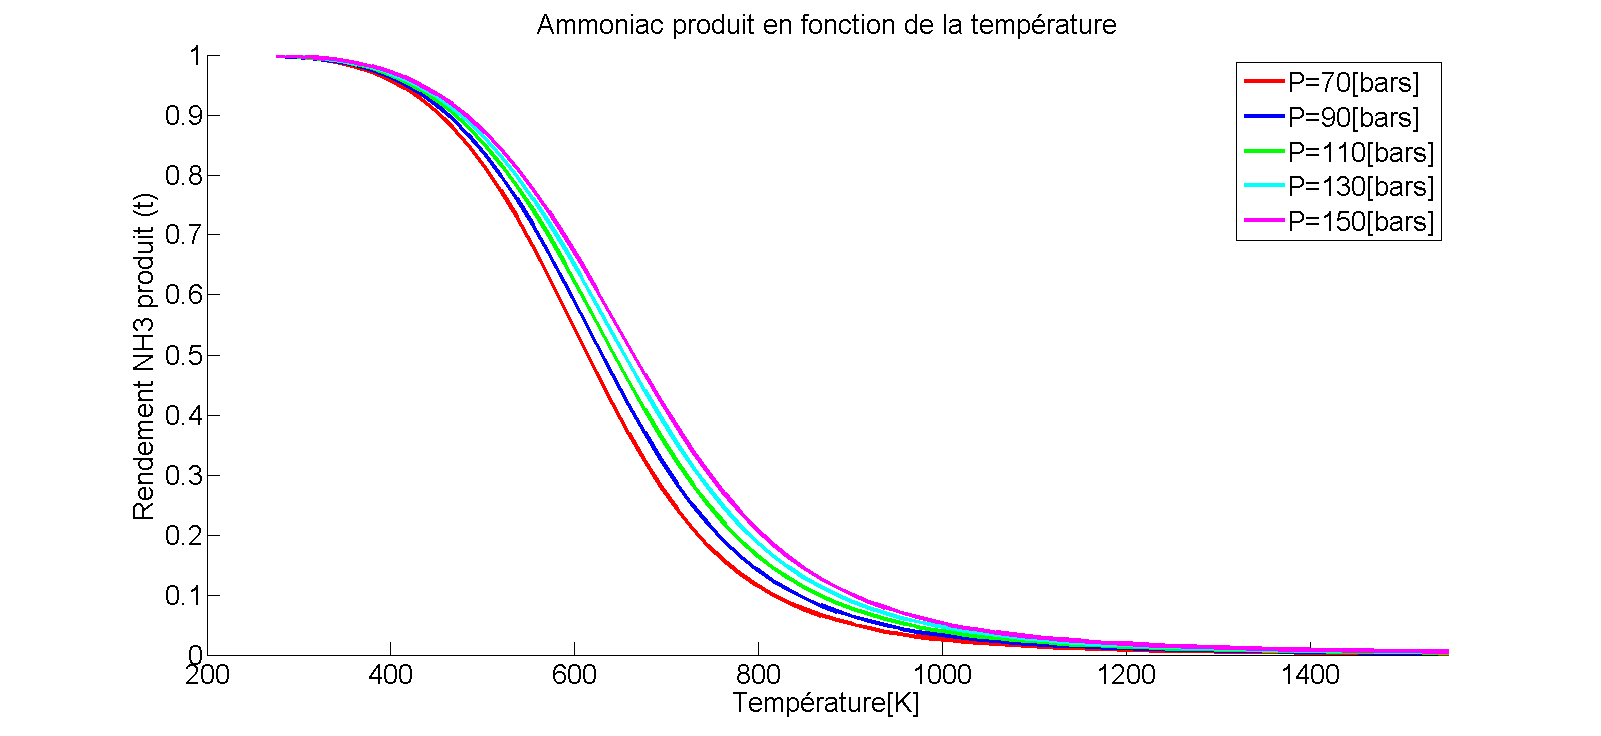
\includegraphics[scale=0.2]{GrapheNH3T.png}
 \caption{Evolution du rendement en fonction de la température}
 \label{scheme2}
\end{figure}


Nous sommes rapidement arrivé au constat que l'augmentation du rendement était causé par une hausse de pression et une diminution de température. La présence d'un catalyseur nous nécessitait une température réactionnelle de \unit{400}{\celsius}, nous avons donc décidé de fixer notre température réactionnelle à \unit{500}{\celsius} (Argument? On a pas cherché pour la vitesse réactionnelle). Pour la pression, ne sachant pas comment majorer la valeur de cette dernière, nous avons décider de la fixer à 150 bars sur bases de nos recherches (Flowshheet? indiquait combien environ? Celui pour la Hazop). Malgré celà nous avons remarqué que pour une pression de 150 bars à une température de \unit{500}{\celsius}, notre rendement n'était seulement que de 25 pourcents. Nous avons alors pensé à un système de réinjection des réactif en excès et avons établi un nouveau bilan de masse pour la réaction (cfr annexe). 

\end{document}